\chapter{Desenvolvimento Teórico}

\section{Astrofografia}

A astrofotografia é um ramo da astronomia e da fotografia que combina toda a ciência envolvida na documentação e registro de estrelas, constelaçoes, planetas, meteoros, etc.; com a arte da fotografia. Dentro da astrofotografia, existem variantes de fotografia como planetária, solar e céu profundo \cite{livro:astropratica}. Além disso, existem diferenças entre a astrofotografia praticada profissionalmente por cientistas, em grandes telescópios, da praticada por amadores. Porém, ambas as atividades são importantes e se complementam.

As fotografias capturadas por telescópios profissionais possuem vantagens no fato de que essas imagens conseguem uma grande ampliação, foco e definição, devido aos grandes espelhos que compõe suas montagens. Porém, isso se torna um problema para a captura de imagens mais amplas e conseguir observar outros detalhes; essas fotografias são registradas em sua maioria por astrofotografos amadores \cite{livro:astropratica}.

Além disso, a astrofotografia amadora também precisa de equipamentos que, no Brasil, custam um preço que acaba afastando uma boa parcela da população para a prática da observação celeste. 

\subsection{Equipamentos}

Além de uma câmera e uma lente, existem alguns equipamentos periféricos que são fundamentais para a prática da astrofotografia: Tripé e Disparador para a câmera. O tripé é responsável por manter a câmera estável durante o registro das estrelas; o Disparador tem a função de operar a câmera remotamente para evitar que haja o operador faça a câmera tremer ao apertar algum botão e/ou também permitir a utilização do modo \textit{Bulb} das DSLR. O modo \textit{Bulb} consiste em permitir um controle total do tempo de exposição pelo operador \cite{book:bbcsky}.

\subsubsection{Câmeras}

DSLR e Mirrorless. \cite{man:vanessacameras}

\subsubsection{Lentes}

Lentes são um equipamento acoplado no corpo da câmera que é responsável por ordenar a luz que entra no sensor das câmeras. As lentes podem ser rígidas no corpo da câmera no caso de modelos semiprofissionais e compactos; ou podem ser removíveis para o caso de modelos profissionais. Nesse último caso, as lentes removíveis são itens que podem ser obtidos por escolha do fotógrafo e existe uma variedade de modelos.

Esses modelos podem ser lentes fixas ou zoom. O primeiro é um modelo de lente que possui uma distância focal fixa, conseguindo ler apenas um ângulo de visão único. Já as lentes \textit{zoom} permitem uma variação na distância focal o que acaba gerando o \textit{zoom} óptico \cite{man:claudia7licoes}. 

\paragraph{Distância Focal}

A distância focal de uma lente é um fator medido em milímetros e é o fator que determina seu ângulo de visão. Quanto maior ele for, mais fechado será o ângulo de visão, gerando um zoom. Do contrário, quanto menor for a distância focal, maior será o ângulo de visão e consequentemente menor será o zoom da lente. A figura \ref{fig:focaldistance} ilustra essa relação da distância focal \cite{man:claudia7licoes}.

\begin{figure}[htb]
	\centering
	\caption{Efeito de zoom gerado pela variação da distância focal}
	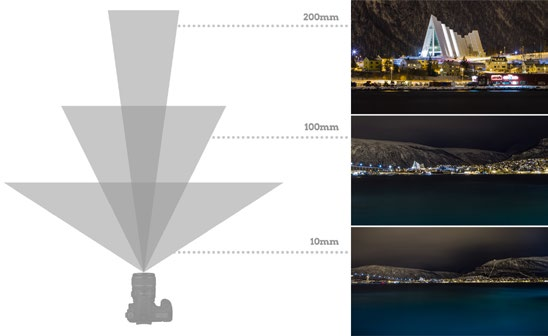
\includegraphics[width=0.7\linewidth]{figuras/claudia-distanciafocal}
	\label{fig:focaldistance}
	\fonte{\cite{man:claudia7licoes}}
\end{figure}

Em um contexto de astrofotografia, lentes mais abertas são úteis para capturar a Via Láctea (Figura \ref{fig:vialactea4mmSony}). Para fotografias de constelações, nebulosas e planetas distantes da Terra, é necessário uma lente mais fechada, que possibilite o enquadramento com o zoom necessário. (Figura \ref{fig:jupiterSony})

\begin{figure}[!htb]
	\centering
	\caption{Fotografia da Via Láctea com lente \textit{zoom} em configuração de 4mm.}
	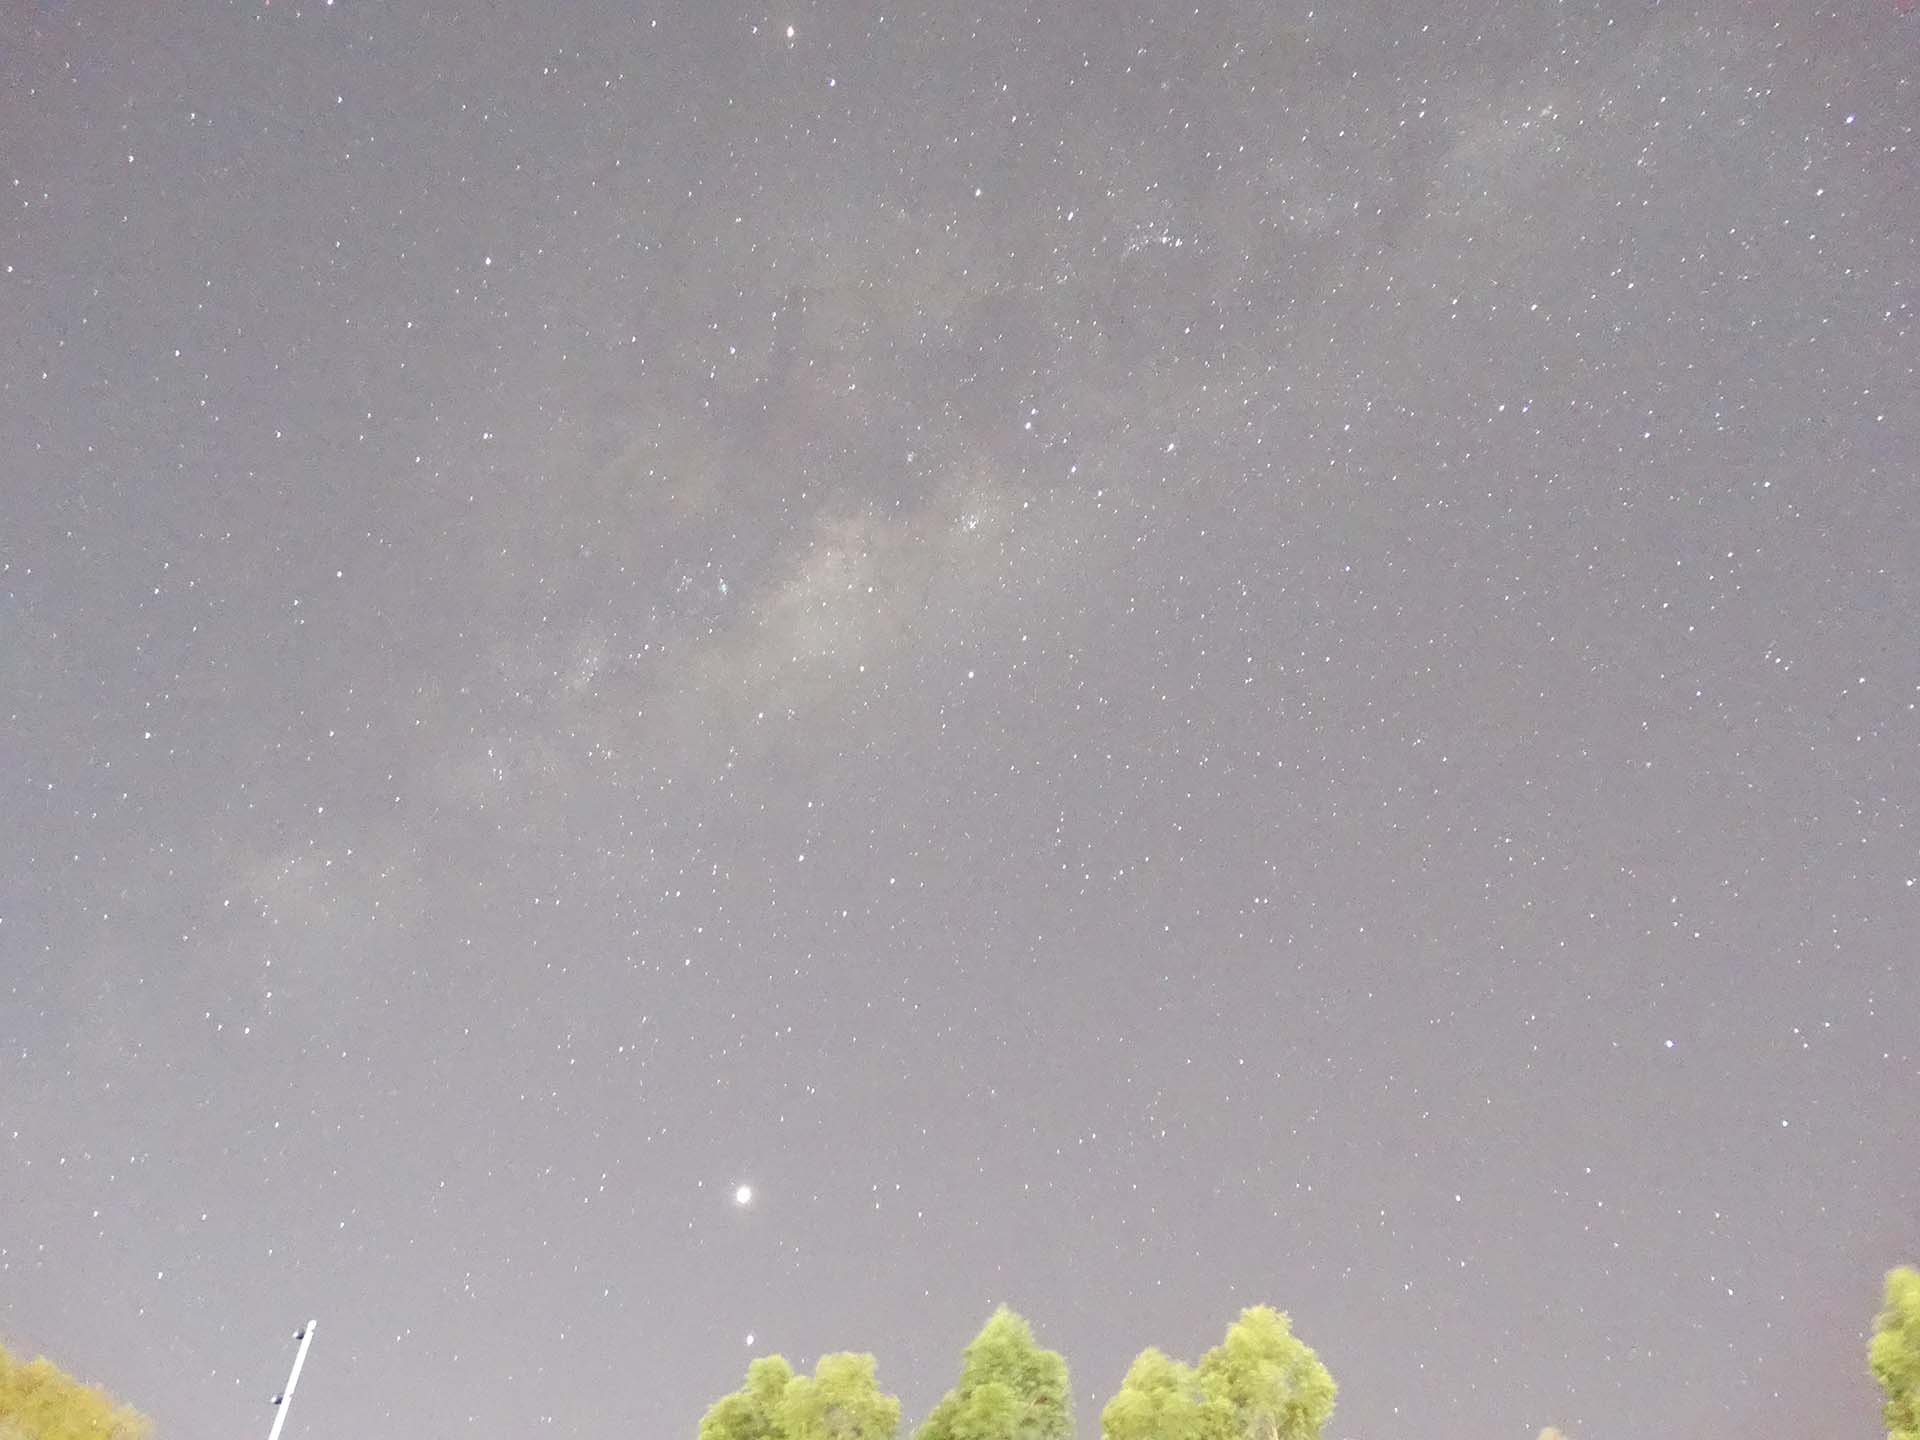
\includegraphics[width=0.7\linewidth]{figuras/vialactea4mm}
	\label{fig:vialactea4mmSony}
	\fonte{Autor}
\end{figure}

\begin{figure}[!htb]
	\centering
	\caption{Fotografia de Júpiter e as Luas de Galileu com lente \textit{zoom} em configuração de 205mm.}
	\includegraphics[width=0.2\linewidth]{figuras/jupiter205mm_Luas}
	\label{fig:jupiterSony}
	\fonte{Autor}
\end{figure}

\subsection{Exposição}

A exposição de uma imagem se refere a quantidade de luz captada pelo sensor da câmera. Uma imagem muito clara é uma imagem superexposta, um caso onde o sensor recebeu muita luz; ao contrário, uma imagem subexposta é uma fotografia escura que recebeu pouca luz. Existem 3 parâmetros configuraveis em uma câmera profissional que são determinantes para a quantidade de luz a ser captada pelo sensor e também para a qualidade da foto final \cite{site:eduardoemonica}. De forma geral, conseguir a exposição ideal é o principal desafio da astrofotorafia de céu profundo \cite{livro:astropratica}.


\subsubsection{Velocidade}

Para captar uma imagem, a câmera possui um dispositivo que permite a entrada de luz no sensor interno que capta a imagem. O tempo que a câmera permite a passagem de luz determina a velocidade do disparador dela. Uma fotografia de longa exposição significa que a câmera permaneceu captando luz por um longo intervalo de tempo \cite{book:bbcsky}. Porém, não é possível abusar de longas exposições em alguns casos pois a imagem pode sair "borrada" (Figura \ref{fig:velocidade}); uma pessoa correndo precisa ser fotografada em uma fração de segundo, uma paisagem, ao contrário, pode ser capturada durante mais de um segundo se a câmera estiver imóvel em um tripé.  

\begin{figure}[!htb]
	\centering
	\caption{Impacto da Velocidade de captura para objetos em movimento}
	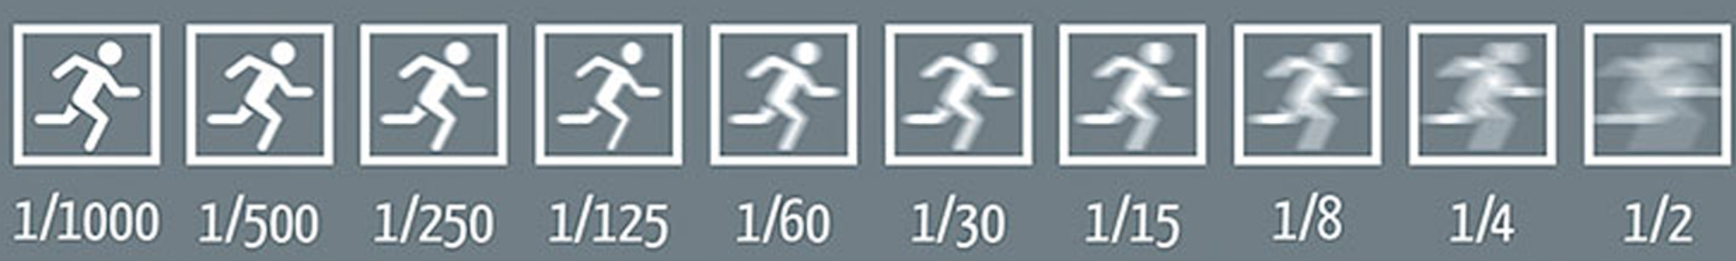
\includegraphics[width=0.7\linewidth]{figuras/velocidade}
	\label{fig:velocidade}
	\fonte{Adaptado de \cite{site:eduardoemonica}}
\end{figure}

\subsubsection{Abertura}

Esse é o diâmetro da abertura da lente, que permite a passagem de luz para o sensor (Figura \ref{fig:abertura}). Isso determina um valor "f/número". Um baixo "f/número" como f/1.8, indica um alto valor de abertura e significa dizer que a câmera irá receber mais luz \cite{book:bbcsky}. A abertura também impacta na profundidade de campo (Figura \ref{fig:profundidade}), o que significa que um valor baixo também apresenta o ônus da dificuldade de focar em objetos.

\begin{figure}[!htb]
	\centering
	\caption{Variações de Abertura de uma lente}
	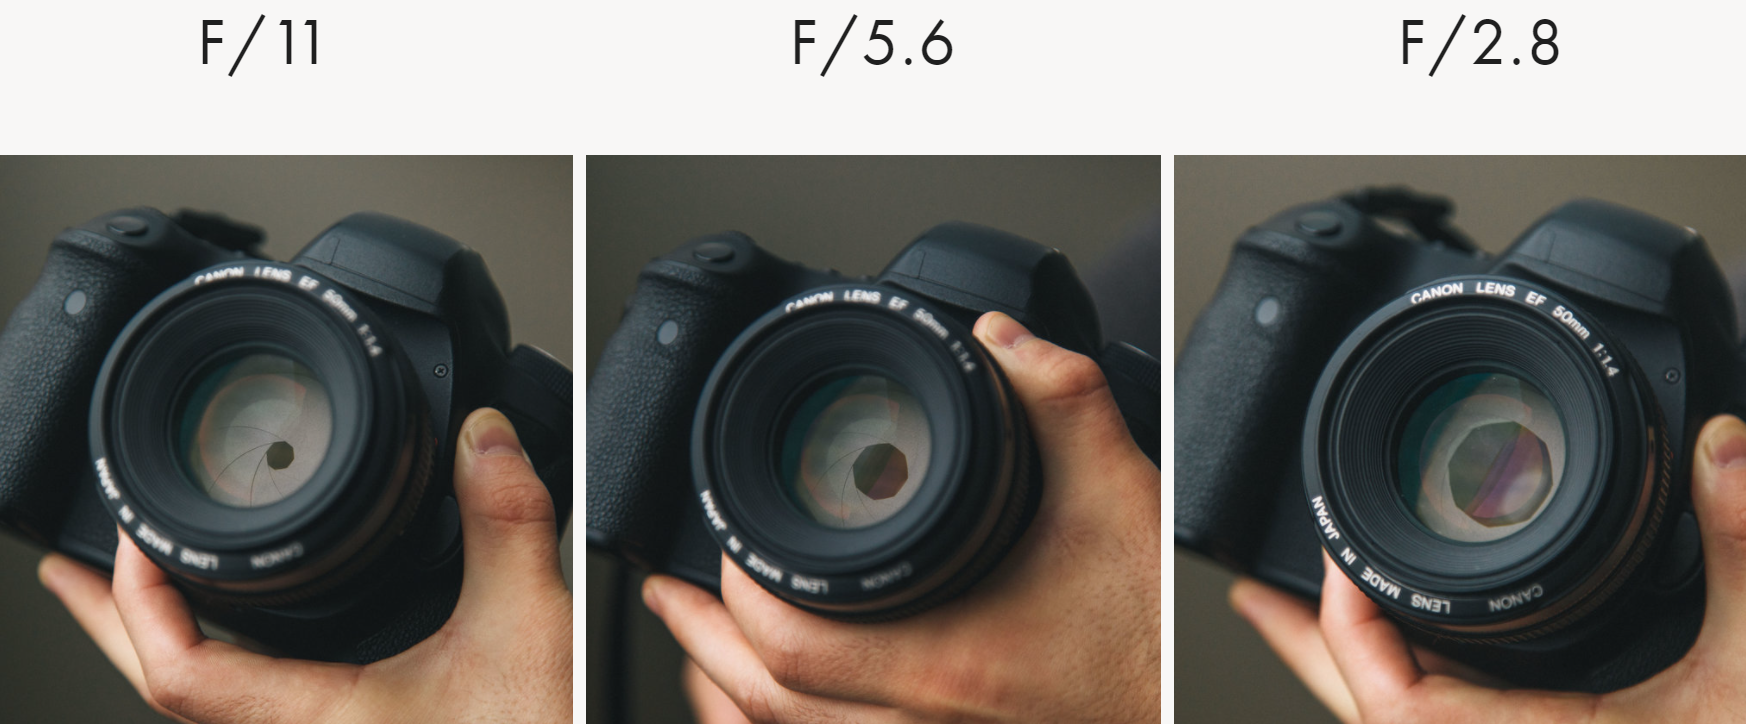
\includegraphics[width=0.7\linewidth]{figuras/abertura}
	\label{fig:abertura}
	\fonte{Adaptado de \cite{site:eduardoemonica}}
\end{figure}

\begin{figure}[h]
	\centering
	\caption{Impacto da abertura na profundidade de campo}
	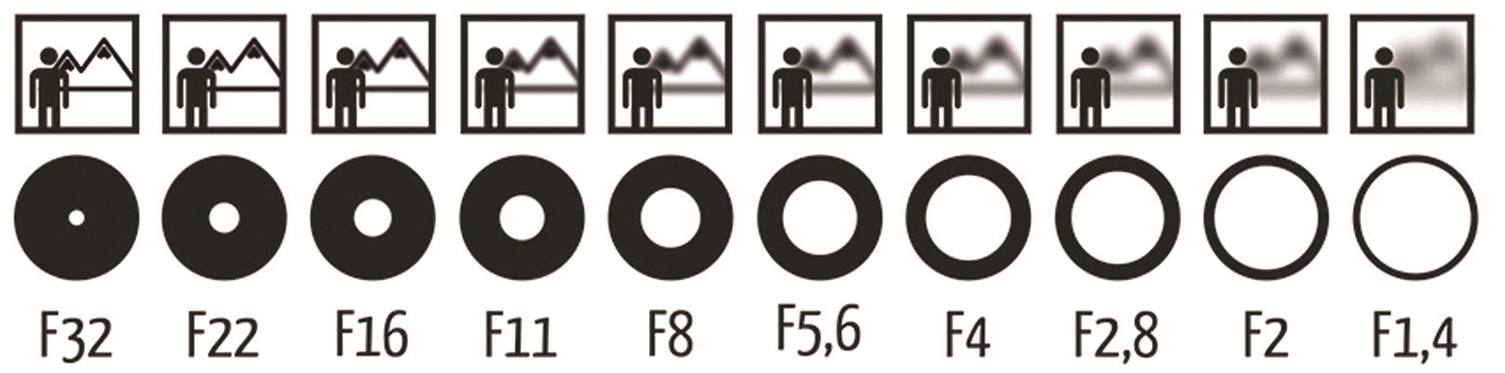
\includegraphics[width=0.7\linewidth]{figuras/profundidade}
	\label{fig:profundidade}
	\fonte{Adaptado de \cite{site:eduardoemonica}}
\end{figure}

\subsubsection{Sensibilidade (ISO)}

O ISO é um padrão internacional para a semsibilidade do sensor das câmeras. Essa sembilidade também é configurável no sistema da câmera no momento da fotografia. Um valor baixo de ISO significa que o sensor precisa de mais tempo de exposição para captar mais luz, ao mesmo tempo que reduz o ruído na imagem. (Figura \ref{fig:iso})
Um valor de ISO alto como 3200 implica que a imagem final terá muito ruído, mas possibilita que ela seja registrada com um baixo tempo de exposição \cite{book:bbcsky}. O ruído agregado pelo ISO também acaba prejudicando a fotografia reduzindo o contraste e saturação das imagens, o que também pode levar a posterização, implicando no comprometimento total da fotografia pois a foto perde resolução e criam-se falhas nos pixeis da imagem.


\begin{figure}[!htb]
	\centering
	\caption{Variações do ISO e o ruído agregado}
	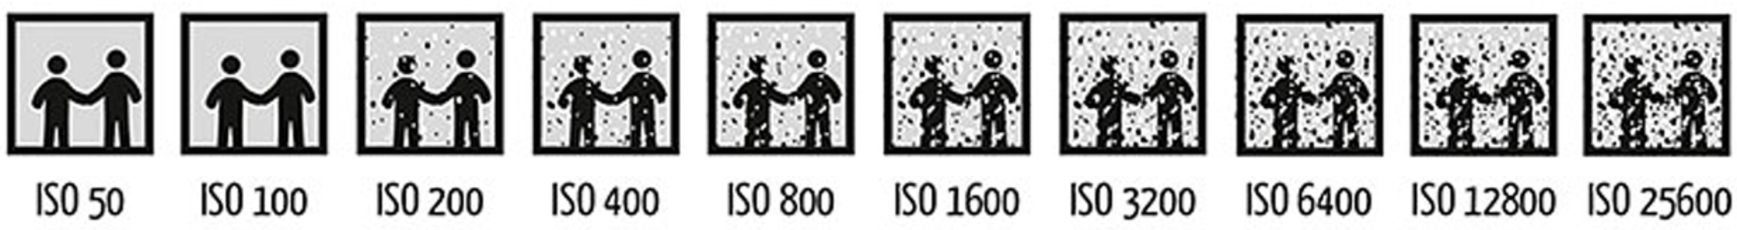
\includegraphics[width=0.7\linewidth]{figuras/ISO}
	\label{fig:iso}
	\fonte{Adaptado de \cite{site:eduardoemonica}}
\end{figure}

\subsection{Formatos de Arquivos}

As câmeras profissionais possibilitam salvar as imagens em diferentes formatos de arquivos, que inclui formato RAW, JPG e Ambos os formatos. Os arquivos JPG são uma versão reduzida dos formatos RAW, onde se aplica um algoritmo de compressão de imagens que acaba gerando perca de informações. Desse modo, arquivos RAW possuem a informação pura do sensor, sem nenhum tipo de compactação e acabam sendo muito pesados porém permitem uma pós produção mais precisa que acaba finalizando em uma imagem com mais qualidade e detalhes \cite{book:bbcsky}.

\subsection{Rastro de Estrelas}

O movimento de rotação da terra gera um movimento aparente no céu. Ao realizar uma fotografia de longa exposição, esse movimento será visível criando o efeito de Rastro de Estrelas ou \textit{star-trail}. (Figura \ref{fig:startrail_example})

\begin{figure}[!htb]
	\centering
	\caption{Fotografia com a captura de um \textit{Star Trail} (Rastro de Estrelas)}
	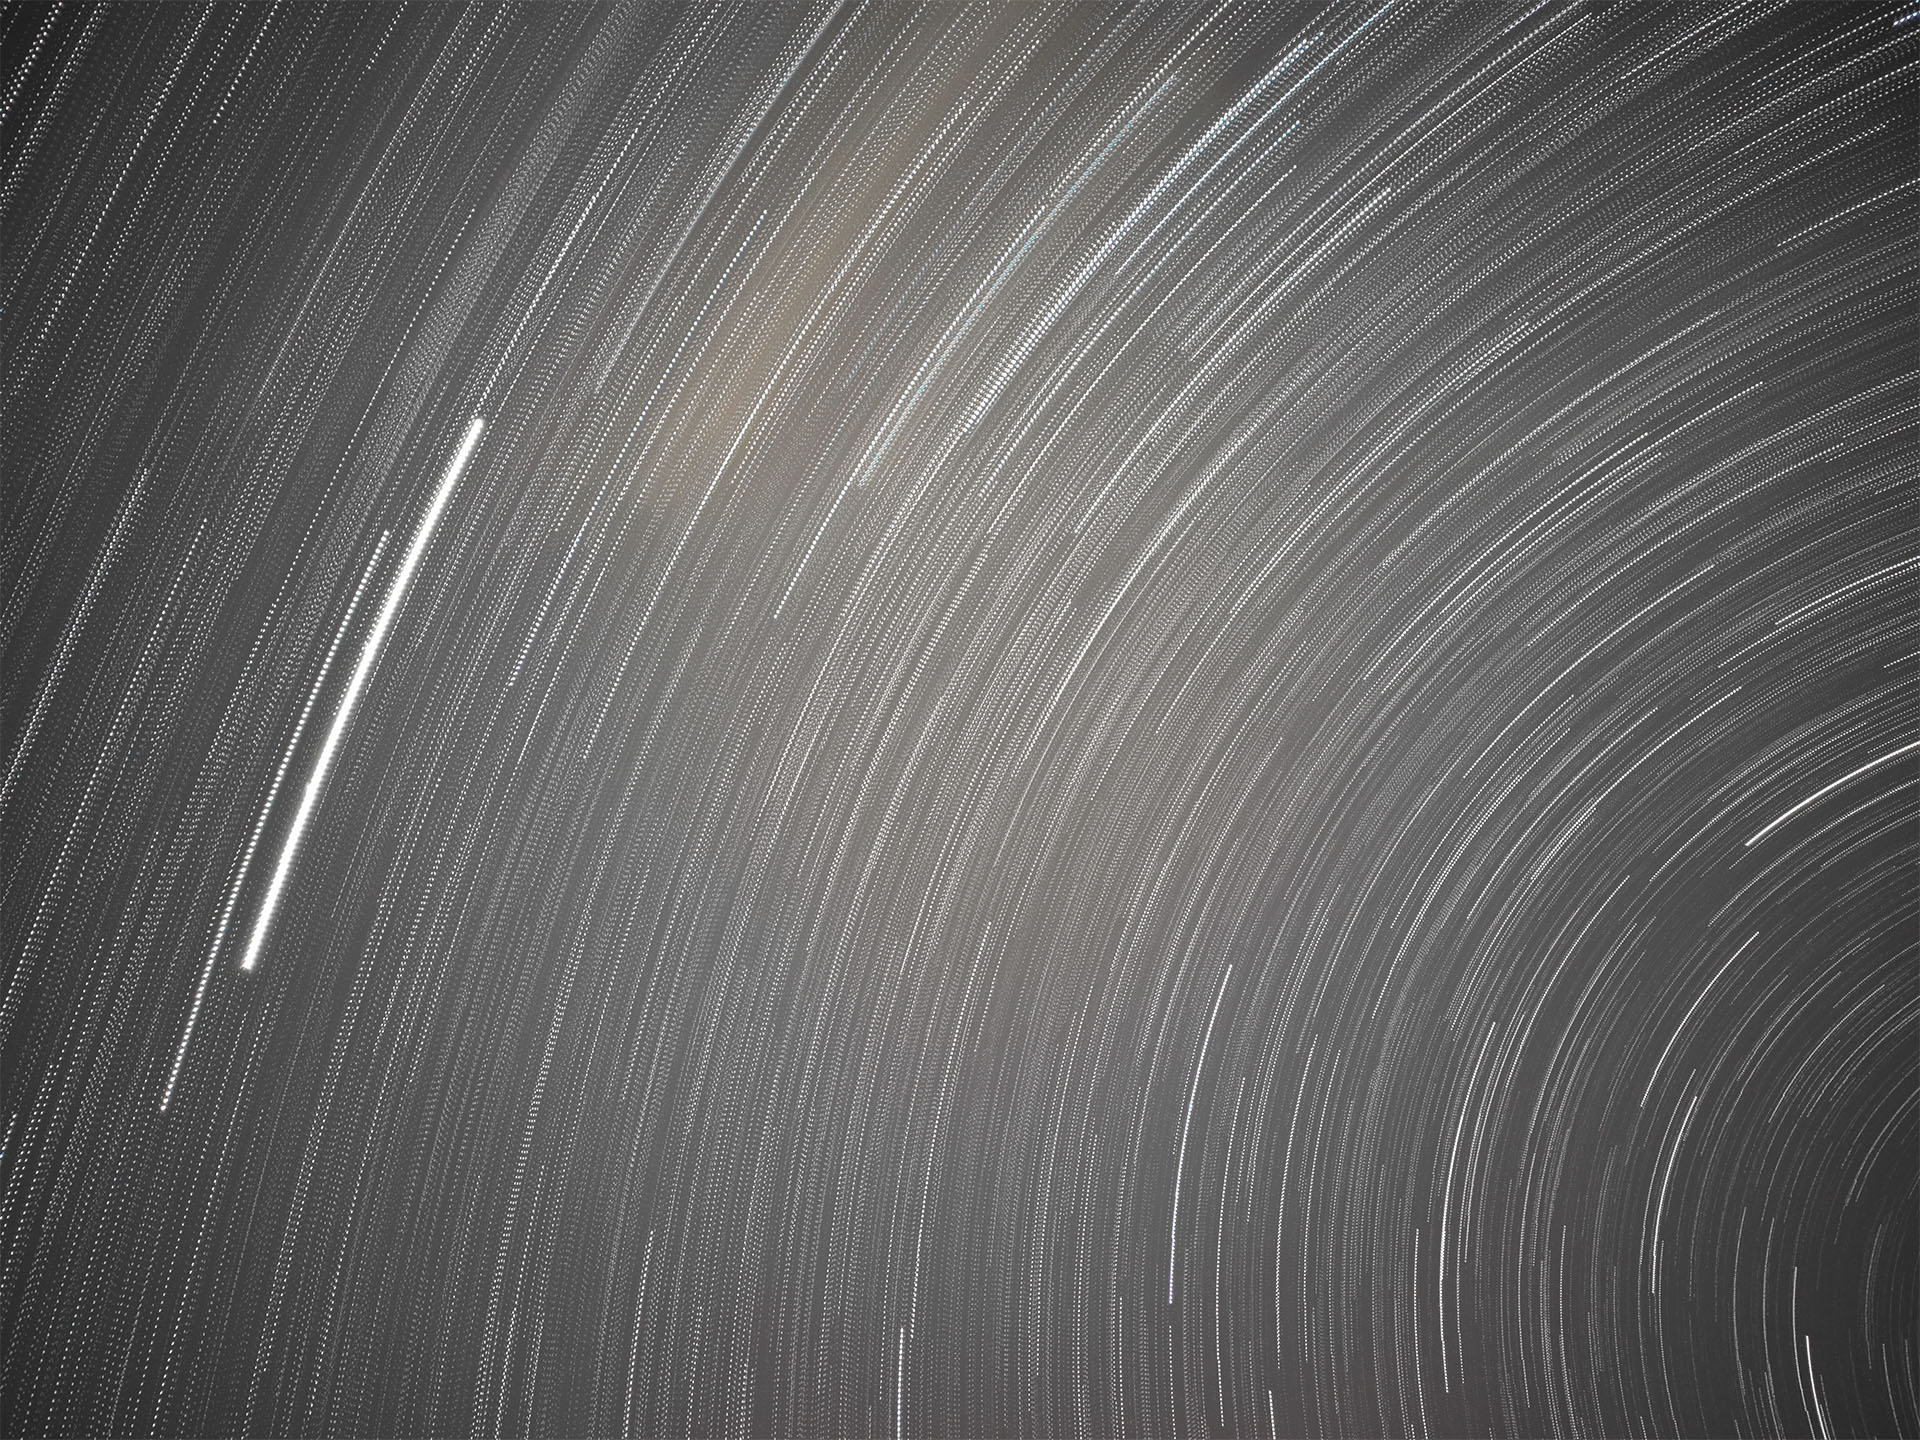
\includegraphics[width=0.7\linewidth]{figuras/startrail_example}
	\label{fig:startrail_example}
	\fonte{Autor}
\end{figure}

\subsection{Empilhamento de Fotos}

O fenômeno de Star Trail gera a necessidade do uso de ferramentas para compensar o movimento da terra e permitir uma fotografia de longa exposição sem que se crie rastro. Essa compensação pode ser feita por meio de software, realizando-se o empilhamentos de fotos de curta exposição \cite{livro:astropratica}.

O empilhamento consiste na junção de multiplas imagens capturadas com a câmera montada em um tripé ou em uma montagem motorizada, que possibilita o somatório da luz capturada com essas fotos. Esse método de processamento é relevante para qualquer tipo de astrofotografia e possibilita a redução de ruído usando imagens de calibração \cite{book:bbcsky}. Existem inúmeros programas capazes de realizar esse processo como Deep Sky Stacker, Sequator entre outros.

A combinação das imagens no pós processamento não gera uma imagem mais luminosa ou mais colorida, o objetivo da combinação é o aumento da Relação Sinal Ruído (SNR). A única forma de gerar uma imagem final com mais luz e cores é realizando uma sequência de fotografias com um maior tempo exposição \cite{man:deepskystackerBetterImages}. As figuras \ref{noCalibration} e \ref{withCalibration} comparam o resultado final de uma imagem que passou pelo processo de empilhamento. 

\begin{figure}[!htb]
	\centering
	\caption{Efeito da combinação de imagens.}
	\begin{subfigure}[b]{0.49\textwidth}
		\centering
		\caption{Imagem original}
		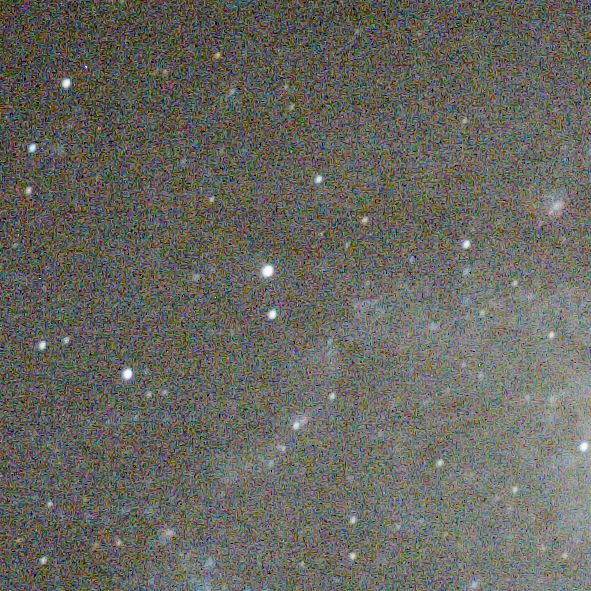
\includegraphics[width=\textwidth]{figuras/Stack_1}
		\label{noCalibration}
	\end{subfigure}
 	\hfill
 	\begin{subfigure}[b]{0.49\textwidth}
 		\centering
	 	\caption{Empilhamento de 32 imagens}
	 	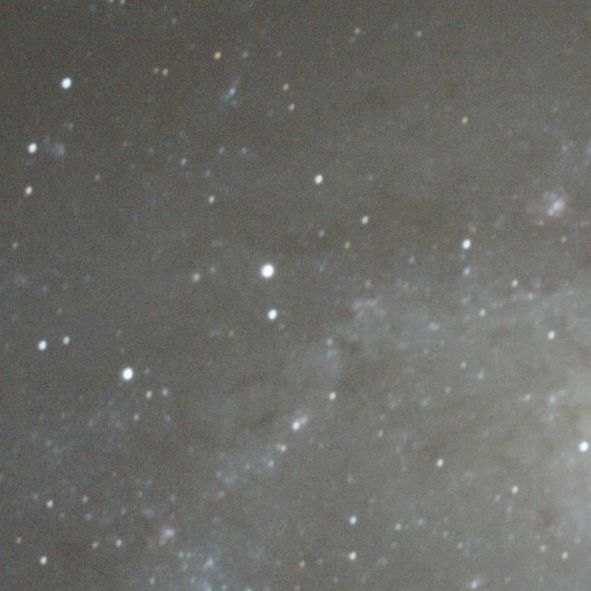
\includegraphics[width=\textwidth]{figuras/Stack_32}
	 	\label{withCalibration}
	 \end{subfigure}

	\fonte{\cite{man:deepskystackerBetterImages}}
\end{figure}


\subsubsection{Imagens de Calibração}

As fotografias registradas sobre um alvo celeste são chamadas de \textit{Light Frames} e estas podem ser empilhadas como escrito anteriormente. No entanto, é possível realizar um processo de calibração do empilhamento, fornecendo imagens de calibração. \cite{man:deepskystackerfaq}
O processo é feito combinando fotos chamadas de \textit{Dark Frames},\textit{ Bias Frames}, \textit{Flat Frames} e \textit{Dark Flat Frames} (Não muito Utilizado). Essas imagens são extras e precisam ser fotografadas com a câmera em condições específicas numa quantidade razoável e posteriormente adicionadas no software durante o processo de empilhamento 
\cite{man:deepskystackerBetterImages}. O resultado final entregue pelo software será uma imagem final calibrada como demonstra o diagrama da Figura \ref{fig:calibrationDeepSkyStacker}.

\begin{figure}[!htb]
	\centering
	\caption{Diagrama do Processo de calibração do empilhamento sem o uso de \textit{Dark Flat Frames}}
	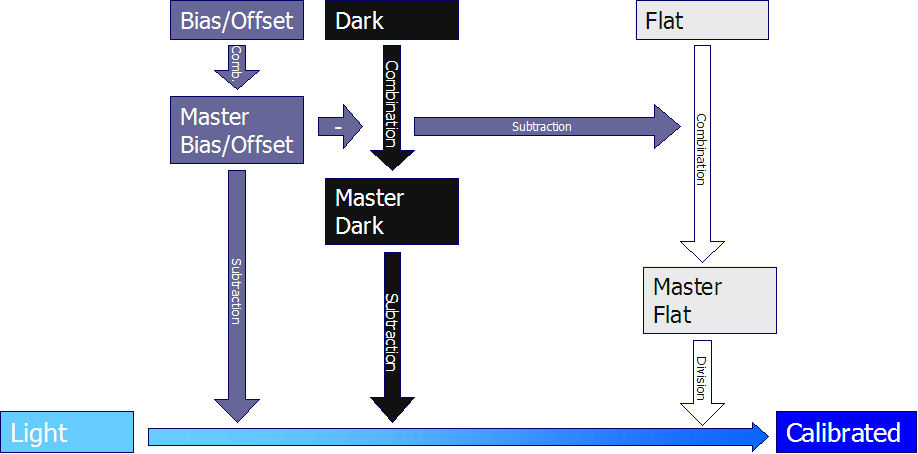
\includegraphics[width=0.7\linewidth]{figuras/Calibration_Alternate1}
	\label{fig:calibrationDeepSkyStacker}
	\fonte{\cite{man:deepskystackerBetterImages}}
\end{figure}


\paragraph{\textit{Dark Frames}}

Os \textit{Dark Frames} são fotografias que indicam ao software o sinal de ruído das fotografias escuras, dadas as condições dos \textit{Light Frames}. São necessárias de 10 a 20 fotos com a lente tampada para criar a calibração, as quais devem necessariamente ser fotografadas com ISO, velocidade e temperatura iguais.\cite{man:deepskystackerfaq}

\paragraph{\textit{Bias (Offset) Frames}}

Os \textit{Bias/Offset Frames} são usados para remover sinais de ruído na leitura dos sensores que captam as imagens. Essas fotografias devem ser caputradas na maior velocidade de obturador possível, com lente tampada, na mesma configuração de ISO dos \textit{Light Frames}. São necessárias cerca de 10 a 20 fotos para que a calibração funcione adequadamente. A temperatura da câmera não é um fator relevante \cite{man:deepskystackerfaq}.


\paragraph{\textit{Flat Frames}}
\textit{Flat Frames} são imagens de calibração capturadas com mesmo ISO das fotos originais colocando uma folha branca na frente do sensor, incidindo luz na folha. Elas tem o objetivo de indicar a vinheta da lente(escurecimento nas bordas da imagem) natural da lente, além da distribuição não uniforme de luz provocada por pó ou riscos na lente. Novamente são necessários de 10 a 20 \textit{frames}
\cite{man:deepskystackerfaq}.


\subsection{Métodos de Rastreamento}

\subsubsection{Alt-Azimutal}
\subsubsection{Equatorial}

\section{Plataformas Equatoriais}

\subsection{Métodos de Alinhamento Polar}

\subsubsection{Ajuste de Azimute}

\paragraph{Localização da Estrela Polar}
Uso de lunetas para alinhamento

\paragraph{Alinhamento com o Polo Norte}
Declinação Magnética

\subsubsection{Ajuste de Elevação}

\subsubsection{Método \textit{Drift}}

\subsection{Soluções Comerciais Existentes}

Existem inúmeras soluções comerciais para o problema proposto, porém todos eles usam uma luneta ou \textit{laser} como método de alinhamento polar. Isso só é possível no hemisfério norte devido a presença da estrela polar. Existem produtos com diferentes especificações e orçamentos. A Tabela \ref{tabela_benchmark} ilustra os principais equipamentos, comparando suas funcionalidades. 

\begin{table}[htb]
	\caption{Comparativo das Soluções de Mercado}
	\begin{tabular}{l|cccc}
		& Nyx Tracker & iOptron & Vixen Optics & SkyWatcher \\ \hline
		Preço (US\$) & 115 & 299 & 399 & 299 \\\hline
		Carga Máxima (kg) & 2.25 & 3 & 2 & 3 \\\hline
		Erro periódico (arcsec) & 115 & 100 & 50 & 50 \\\hline
		Volume $ (cm^2) $ & 155 & 490 & 323 & 220 \\\hline
		Peso (kg) & 0,4 & 1,15 & 0,79 & 0,72 \\\hline
		Alinhamento & \textit{Laser} & \textit{Polar Scope} & \textit{Polar Scope} & \textit{Polar Scope} \\
	\end{tabular}
	\label{tabela_benchmark}
	\fonte{Adaptado de \cite{site:nyxtech}}
\end{table}

Contudo, na realidade brasileira, o preço mostrado passaria ainda por impostos, tornando a compra mais inviável. O Nyx Tracker (Figura \ref{fig:nyxtracker}) é o sistema mais acessível, mas com alinhamento difícil no hemisfério sul.

\begin{figure}[h]
	\centering
	\caption{Nyx Tracker}
	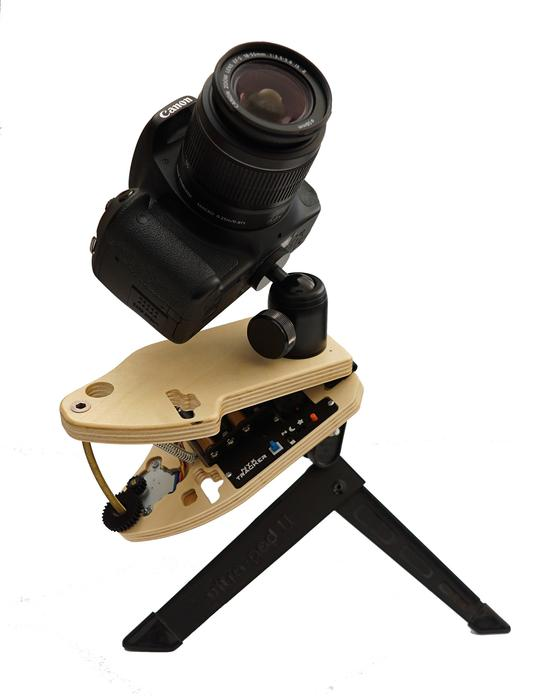
\includegraphics[width=0.3\linewidth]{figuras/nyxtracker}
	\label{fig:nyxtracker}
	\fonte{\cite{site:nyxtech}}
\end{figure}


\section{Objetivos}

Pelo \textit{benchmark} exposto, fixou-se como objetivos o desenvolvimento de uma solução robusta, visualmente elegante, e que consiga se aproximar das propriedades do modelo comercial mais acessível com o custo inferior a 115 dólares. Além disso, deve ter como diferencial um aplicativo que permita uma fácil interação do usuário com o sistema, facilitando o processo de configuração e alinhamento polar.

\section{Protocolos de Comunicação}

\subsection{Serial}
\subsubsection{UART}
Velocidade, Falhas de comunicação, Guidelines de Design de PCB

\subsubsection{I2C}

Endereçamento, Velocidade, Guidelines de Design de PCB

\subsection{Bluetooth}

\section{Sensores e Atuadores}

\subsection{Acelerômetro}
\subsection{Giroscópio}
\subsection{Magnetômetro}

\subsection{GPS}

\subsection{Motor de Passo}

Driver, formas de Acionamento...

\section{Microcontroladores}

\subsection{Arduino Nano}

Justificativa, diagrama do Arduíno

\section{Interface Gráfica}

\subsection{Princípios e Diretrizes}

Os princípios e as diretrizes comumente utilizados em interfaces humano computador giram em torno dos seguintes tópicos: correspondência com as expectativas dos usuários; simplicidade nas estruturas das tarefas; equilíbrio entre controle e liberdade do usuário; consistência e padronização; promoção da eficiência do usuário; antecipação das necessidades do usuário; visibilidade e reconhecimento; conteúdo relevante e expressão adequada; e projeto para erros \cite{BarbosaEtAl2021InteracaoHumanoComputadorExperiencia}.
Esse conjunto de princípios são conhecidos como heurística de Nielsen, pois são aplicáveis em qualquer sistema, independente de casos específicos.

\subsubsection{Visibilidade dos status do sistema}

O sistema deve sempre manter o usuário atualizado sobre as condições de operação com uma taxa de atualização condizente para a informação. Ao informar o status da bateria, por exemplo, o usuário do \textit{smartphone} consegue predizer quanto tempo de uso ainda terá e irá conseguir manejar sua interação com base nessa previsibilidade \cite{site:nielsen}.

\subsubsection{Comunicar-se com o mundo real}
O Projeto tem que se comunicar com o usuário na língua do usuário. Se um brasileiro não sabe inglês, ele "ficará perdido" nos Estados Unidos. Da mesma forma, o desenvolvedor não pode assumir que o usuário entenderá o aplicativo somente pelo fato do desenvolvedor ter feito algo que ele próprio entenda. É sempre recomendado conferir a linguagem do sistema com um conjunto grande de pessoas para evitar mal entendidos.

Quando o usuário não entende a língua do sistema, ele se sente afastado e irá deixar de usar a plataforma. É interessante que a plataforma tenha \textit{designs} semelhantes com objetos do mundo real, dessa forma, o usuário se sente "contemplado" e consegue facilmente fazer a conexão entre o mundo real e a plataforma \cite{site:nielsenRealWorld}.

\subsubsection{Liberdade de Controle do Usuário}

Por vezes, a pessoa que está realizando um processo em um sistema pode cometer um engano. Esse evento pode levar a situações de erro que não devem comprometer a experiência. Por isso, os usuários precisam de uma “saída de emergência” claramente marcada para sair do estado indesejado. Isso reduz a sua ansiedade e o medo de errar, pois ele sabe que os erros podem ser conternados \cite{BarbosaEtAl2021InteracaoHumanoComputadorExperiencia}.

\subsubsection{Consistências e Padrões}

É importante que o sistema mantenha uma consistência entre suas telas, ou mesmo em grandes plataformas, ou seja, que os múltiplos programas tenham o mesmo padrão, com funções localizadas no mesmo lugar, com nomes similares e com um \textit{disign} similar. Exemplo disso são as telas dos aplicativos do Google Docs: todos possuem o mesmo extilo de menu. Idem para o Microsoft Office.

A consistência também se extende aos ícones. O ícone que representa um botão, por exemplo, é importante que seja consistente em extilo com os demais. Eles podem ser mais preenchidos, mais \textit{clean}, mais neturos ou mais suaves. O que importa nesse caso, é que sejam todos padronizados \cite{site:nielsenIcon}.


\subsubsection{Prevenção de erros}

Uma forma de prevenção é oferecer sugestões numa caixa de pesquisa por exemplo. Em situações de rotina, como disparar um lembrete, a tela de criação pode oferecer uma sugestão padrão de um modelo que faça sentido para o usuário. Para evitar corrupção de dados pelo usuário durante o cadastro, é possível sugerir ao usuário o preenchimento de números de forma truncada, fazendo o pós processamento para ler o número corretamente.

\subsubsection{Relembrar o usuário é mais fácil do que o usuário relembrar}

Quando o usuário precisa repensar sobre algo incomum na memória, ele despende muito tempo. Então, quando a plataforma exige uma lembrança do usuário para entender algo, isso limita a experiência e incorre em perda de tempo ou confusão.

Por isso, é mais interessante realizar a exigência com uma possível sugestão de resposta correta. A recognição de algo é muito mais prática para a mente humana, pois ao mostrar para o cérebro algo relacionado com o que precisa lembrar-se, dispara-se a memória de forma mais efetiva. Dar uma pista para o cérebro é mais eficiente do que simplesmente perguntar sem oferecer nada \cite{site:nielsenRecall}.

\subsubsection{Torne o sistema flexível e eficiente}

Atalhos, personalização e customização. Com esses 3 fatores é possível melhorar a usabilidade para aqueles que não são mais novatos no \textit{software} e isso ajuda a manter esses usuários ativos. Um fotógrafo experiente, que está acostumado com os atalhos de teclado nos aplicativos da Adobe, teria muita dificuldade se o teclado viesse a falhar, pois a mente já assimilou os atalhos mais usados e eles fazem diferença na velocidade com que o profissional interage com o software \cite{site:nielsenFlexibility}.

\subsubsection{Tenha um projeto minimalista}

Um projeto é minimalista significa usar elementos simples num arranjo onde desenho e a interface combinem de forma agradável sem chamar a atenção de forma desnecessária, colaborando com que o usuário foque somente naquilo que é necessário \cite{site:nielsen}.

\subsubsection{Ajude o usuário a entender e se recuperar de erros}

O usuário precisa entender quando o sistema não está funcionando bem e como fazê-lo voltar à normalidade. As mensagens de erro devem ser expressas de uma forma simples, indicando o possível problema e a solução. 
Cores vermelhas e pretas ajudam a demonstrar o sinal de erro para o usuário \cite{site:nielsenError}.

\subsubsection{Tire dúvidas e documente o sistema}

Existem duas formas de ajudar o usuário e tirar suas dúvidas. A primeira é de forma proativa, onde a aplicação guia o usuário para se familiarizar com a interface. Outra forma é por meio de uma seção com perguntas e respotas, a qual ajuda os usuários a se tornarem mais independetes com a aplicação, resolvendo seus próprios problemas e filtrando os casos que precisam de suporte para a equipe técnica da plataforma \cite{site:nielsenHelpandDoc}.

\subsection{Android}
\subsubsection{Ambiente de Desenvolvimento}

O \textit{Android Studio} é o ambiente de desenvolvimento integrado oficial para a criação de aplicativos \textit{Android} e é baseado no \textit{IntelliJ IDEA}. Ele oferece uma série de Recursos que possibilitam a confecção de um aplicativo: Sistema de compilação flexível baseado em \textit{Gradle}; Um emulador rápido com suporte a vários recursos; ambiente unificado que possibilita o desenvolvimento para qualquer dispositivos Android, incluindo relógios e televisões; integração com \textit{GitHub} para \textit{backup} e documentação do código; entre outras funções que possibilitam análizar o desempenho de um aplicativo em tempo real, bem como fazer updates. \cite{site:androidstudio}

\subsubsection{Linguagens de Programação}

Existem soluções de desenvolvimento Android mais \textit{user-friendly} como \textit{APP Inventor} ou \textit{Kodular}, porém, essas interfaces não garantem ao desenvolvedor um pleno controle do aplicativo, e muitas vezes acabam limitando o projeto da interface. Por isso, usar linguagens de programação nativas é uma abordagem mais interessante para aplicativos mais completos. É possível criar aplicativos com diversas linguagens, mas somente duas são nativas e permitem realizar aplicações que podem usar de todo o poder de processamento de um \textit{smartphone}: Java e Kotlin.

Em 2017, Kotlin foi definido pela Google como sendo a principal linguagem de desenvolvimento Android. A linguagem é muito mais nova que Java, sendo desenvolvida em pela JetBrains. A grande motivação de se usar Kotlin para o desenvolvimento reside no fato de ser uma linguagem segura para prevenção de objetos nulos, operando em paralelo com qualquer código em Java e dando opções de co-rotinas. Além disso, ao comparar dois códigos com a mesma função, um escrito em Java, outro em Kotlin, o segundo pode ser até 40\% mais compacto, o que implica em uma linguagem mais concisa e compreensível entre desenvolvedores. A desvantagem de se usar Kotlin, para este trabalho, é somente a falta de uma comunidade grande, comparando com Java, o que limita o suporte para eventuais problemáticas de desenvolvimento \cite{site:kotlinxjava}.

Dentro do ambiente de desenvolvimento usa-se também linguagem de arquivos XML para a criação de interfaces gráficas (\textit{layouts}), bem como a escrita dos vetores, animações, e arquivos de configuração do aplicativo e temas de \textit{layout}. Para armazenamento de dados dentro do aplicativo, normalmente usa-se um banco de dados que é operado com códigos de consulta \textit{SQL}.

\subsubsection{\textit{Material Design}}
Existem uma série de diretrizes de projeto fornecidas pela Google para guiar o desenvolvimento de aplicativos \textit{Android}. Essas informações são fornecidas principalmente pela biblioteca \textit{Material Design}, que fornece pacotes facilmente implementáveis de \textit{layouts} para aplicações responsivas e padronizadas.

A Biblioteca colabora com o desenvolvedor fornecendo icones, tipografia, cores e componentes gráficos que trazem uma imersão para o usuário de forma simples e minimalista. Os \textit{design} se inspiram no mundo real, facilitando a comunicação com o usuário \cite{site:materialdesign}.



